\section{Water Masses and Mixing}
\label{section:lit_review_mixing}

The ocean is not a homogeneous mass of water but consists of many different water masses. These are classified by their properties, $\theta$ and $S$, and the depth to which they settle. In figure \ref{fig:salinitycrosssectionWOCE} we can see a higher salinity water mass extending in a finger from approximately $5^{\circ}$W at a depth of approximately 1000m. This water mass comes from the Mediterranean outflow. 

\begin{figure}[htbp]
    \centering
    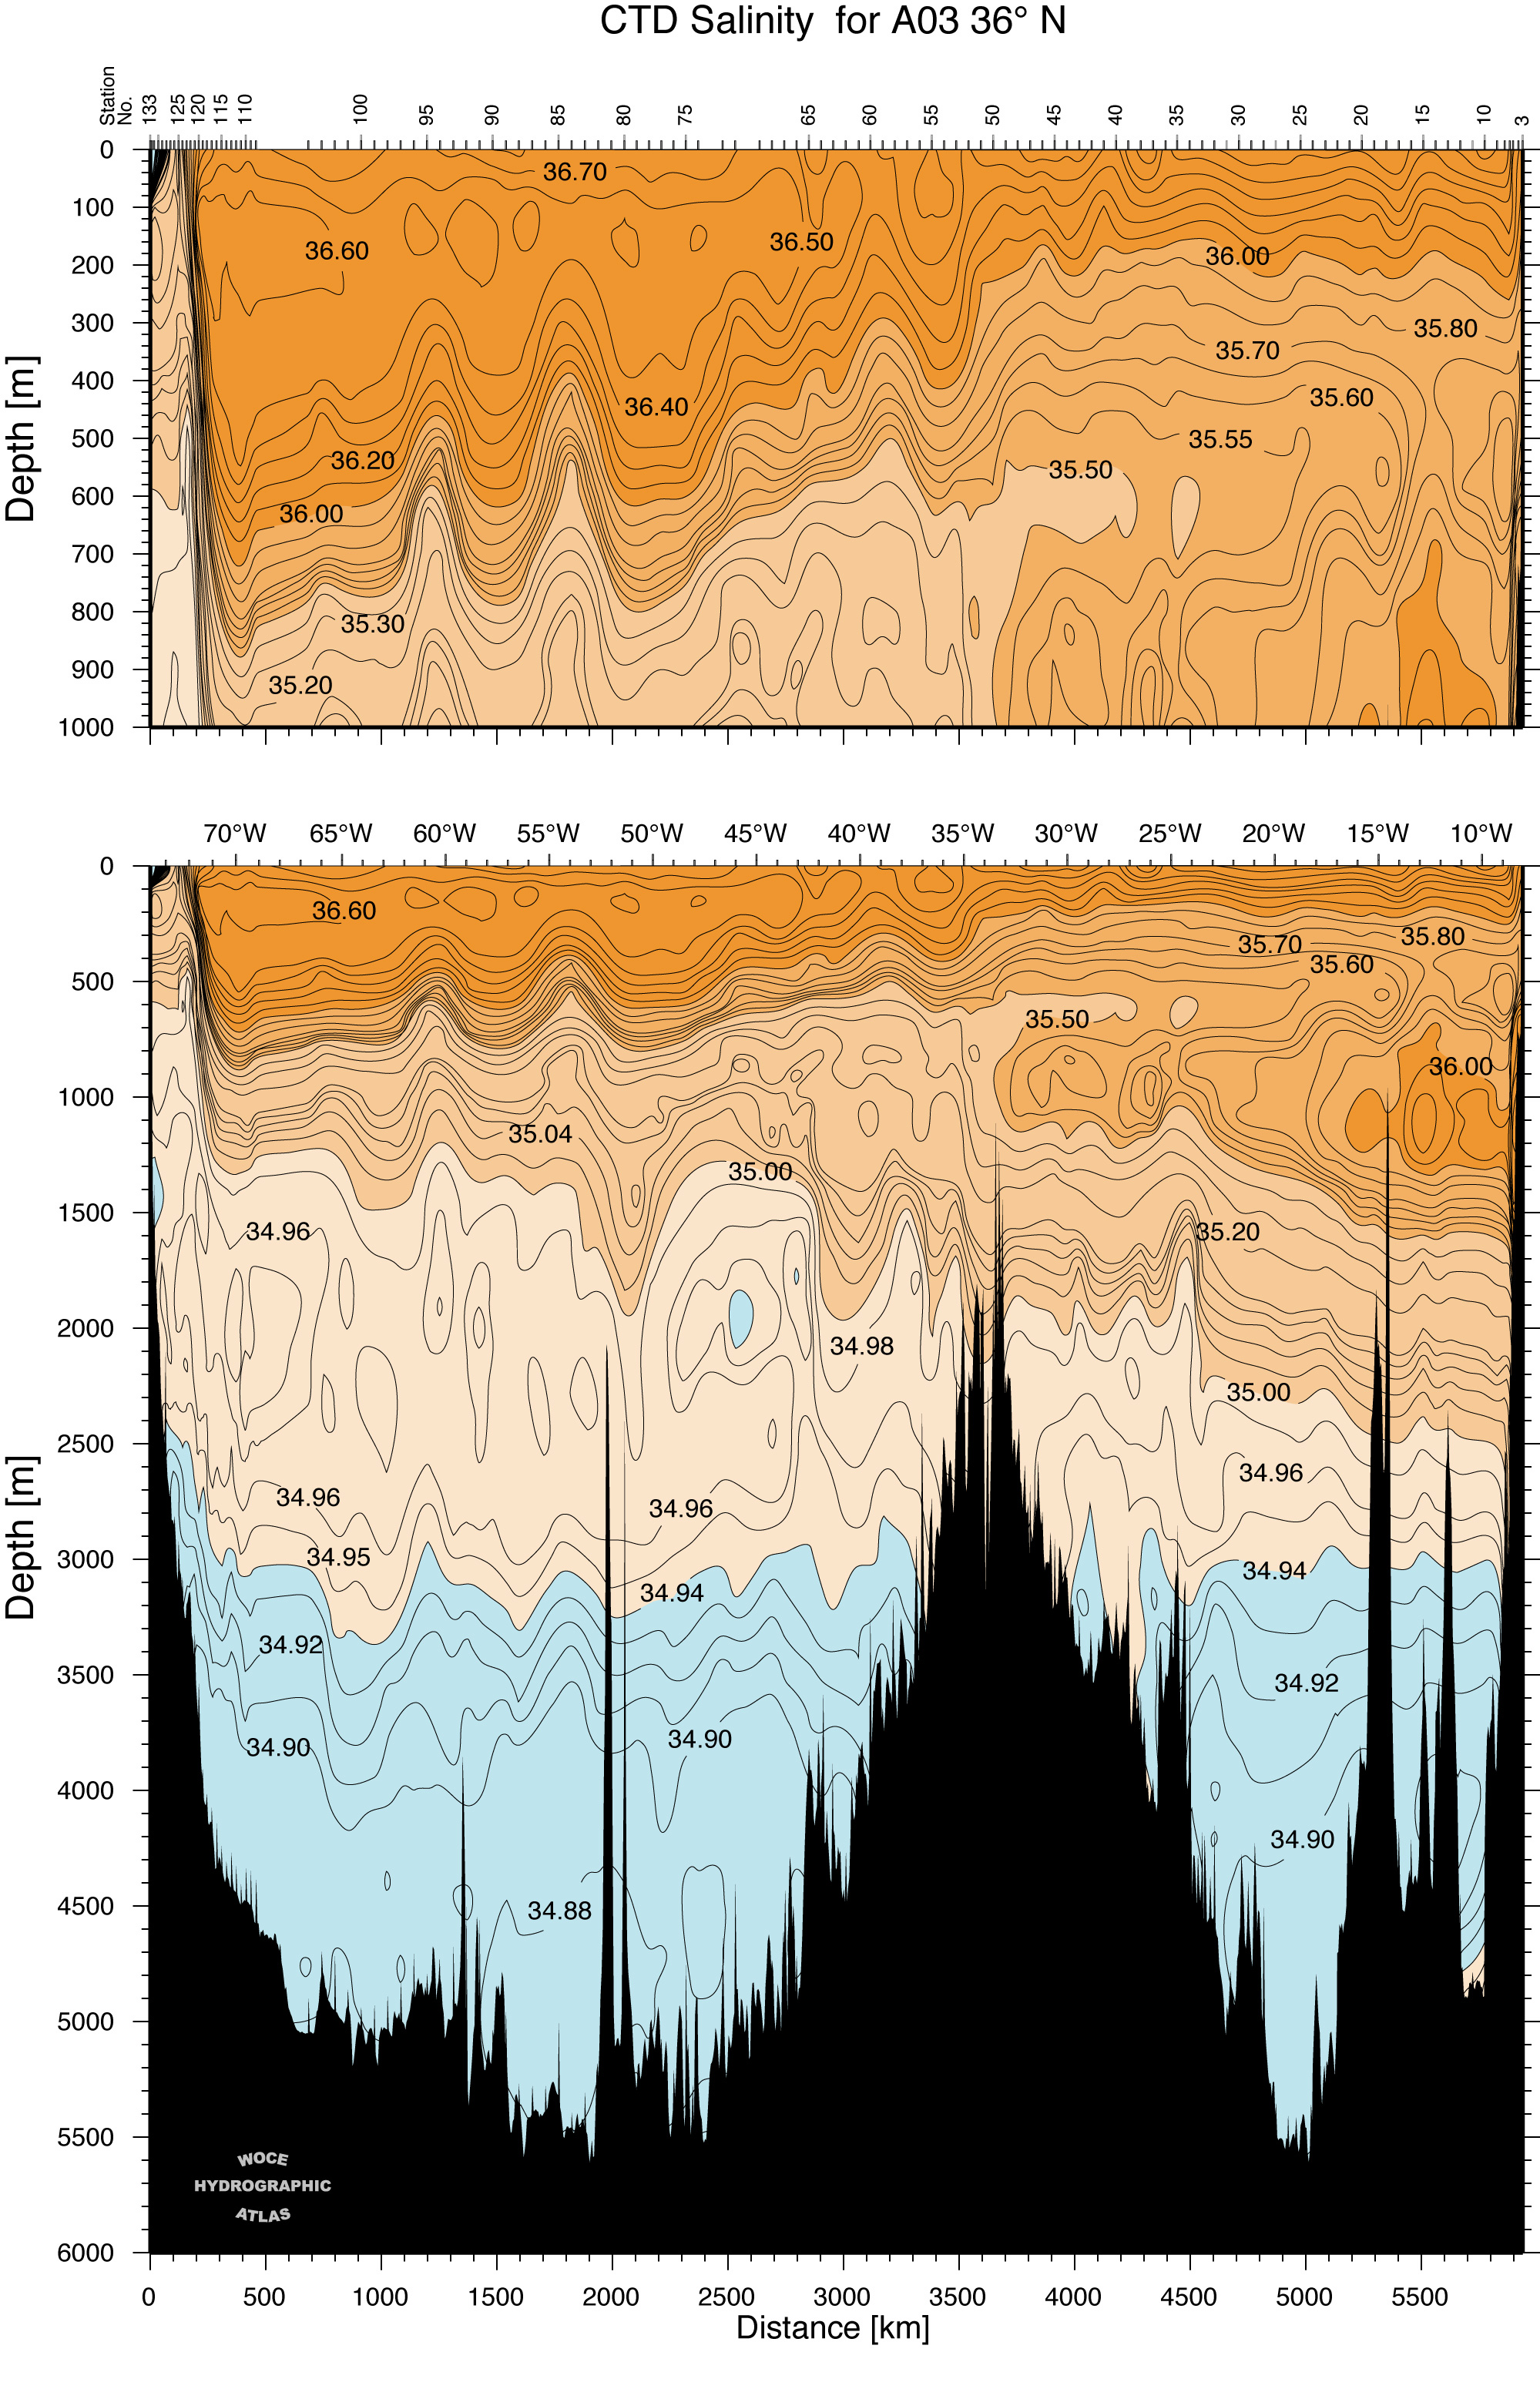
\includegraphics[width = 0.8\textwidth]{A03_CTDSAL}
    \caption{Cross-section of salinity from the WOCE data set along path A03, at 36$^{\circ}$N \citep{WOCEAtlanticAtlas}}
    \label{fig:salinitycrosssectionWOCE}
\end{figure}

In general, water mass properties are set at the surface of the ocean in the winter mixed layer and then retained as they are interred into the ocean interior. However, stirring and mixing does occur in the ocean interior by means of mesoscale eddies \citep{Vallis2017}, \citep{OC4}. 

A key question in oceanography has been to understand the surfaces along which this mixing takes place. 